\documentclass{article}

% Target journal: Molecular Phylogenetics and Evolution
%
% From author guidelines:
%
% Short communications of approximately 3000 words are also accepted. 
% These papers should contain no more than two figures, two tables, and thirty references. 
% A short abstract of fewer than 200 words is acceptable.


% Annotation/feedback commands
\newcommand*\rampal[1]{\textcolor{red}{\textbf{[RSE: #1]}}}
\newcommand*\richel[1]{\textcolor{orange}{\textbf{[RJCB: #1]}}}
\newcommand*\gio[1]{\textcolor{green}{\textbf{[GL: #1]}}}

% Bibliography
\usepackage{natbib}
\bibpunct{(}{)}{;}{a}{}{;}

\usepackage[english]{babel}

% Use 'It was found that something is something (Name 1234)' style
\setcitestyle{authoryear,open={},close={}}

% Affiliations
\usepackage{authblk}
\title{The error in Bayesian phylogenetic reconstruction when speciation co-occurs}

\author[1]{Giovanni Laudanno}
\author[1]{Rich\`el J.C. Bilderbeek}
\author[1]{Rampal S. Etienne}
\affil[1]{Groningen Institute for Evolutionary Life Sciences, University of Groningen, Groningen, The Netherlands}

% Use double spacing
\usepackage{setspace}
\doublespacing

\usepackage{pgf}
\usepackage{hyperref}
\usepackage{verbatim}
  
% Adds numbered lines
\usepackage{lineno}
\linenumbers

\hyphenation{
  BEAST
  Pa-ra-me-ter
  Drum-mond 
  Bayes-ian 
  Mr-Bayes 
  ap-proach-es 
  Rev-Bayes 
  cre-ate
  spe-ci-a-tion-com-ple-tion
  pro-trac-ted
 }

\begin{document}

\maketitle

\begin{abstract}

  % From 'How to construct a Nature summary paragraph'

  % A short abstract of fewer than 200 words is acceptable.

  % One or two sentences providing a basic
  % introduction to the field,
  % comprehensible to a scientist in any discipline.
  The tools for reconstructing phylogenetic relationships between taxonomic 
  units (e.g. species) have become very advanced in the last three decades. 

  % Two to three sentences of
  % more detailed background, comprehensible to
  % scientists in related disciplines.
  Among the most popular tools are Bayesian approaches, 
  such as \\ BEAST, MrBayes and RevBayes, 
  that use efficient tree sampling routines to create a posterior probability distribution 
  of the phylogenetic tree. 
  A feature of these approaches is the possibility to incorporate known 
  or hypothesized structure of the phylogenetic tree through the tree prior. 
  It has been shown that the effect of the prior on the posterior distribution 
  of trees can be substantial. 

  % One sentence clearly stating the general
  % problem being addressed by this particular
  % study.
  Currently implemented tree priors assume that speciation events are independent,
  where we know that speciation can coincide, for example, when trigger by a
  larger geographic change.

  % One sentence summarising the main
  % result (with the words “here we show”
  % their equivalent).
  Here we explore the effects of ignoring 
  speciation co-occurence with an extensive simulation study. 

  % Two or three sentences explaining what
  % the main result reveals in direct
  % comparison to what was thought to be the case
  % previously, or how the main result adds to
  % previous knowledge.

  % One or two sentences to put the results into a
  % more general context.


  % Two or three sentences to provide a
  % broader perspective, readily comprehensible
  % to a scientist in any discipline, may be included
  % in the first paragraph if the editor considers that the accessibility of the paper is significantly enhanced
  % by their inclusion. Under these circumstances, the length of the paragraph can be up to 300 words.
  % (The above example is 190 words without the final section, and 250 words with it).

  We compare the inferred tree to the simulated tree, and find that ....

\end{abstract}

{\bf Keywords:} computational biology, evolution, phylogenetics, Bayesian analysis, tree prior

%%%%%%%%%%%%%%%%%%%%%%%%%%%%%%%%%%%%%%%%%%%%%%%%%%%%%%%%%%%%%%%%%%%%%%%%%%%%%%%%%%%%%%
\section{Introduction}
%%%%%%%%%%%%%%%%%%%%%%%%%%%%%%%%%%%%%%%%%%%%%%%%%%%%%%%%%%%%%%%%%%%%%%%%%%%%%%%%%%%%%%

The computational tools that are currently available 
to the phylogeneticists go beyond the wildest 
imagination of those living four decades ago.
Advances in computational power allowed the first cladograms to be inferred 
from DNA alignments in 1981 (\cite{felsenstein1981}), and  
the first Bayesian tools emerged in 1996 (\cite{rannala1996}),
providing unprecedented flexibility in the setup of a phylogenetic model.

Currently, the most popular Bayesian phylogenetics tools are \\ 
BEAST (\cite{beast}) and its offshoot BEAST2 (\cite{beast2}), 
MrBayes (\cite{mrbayes}) and RevBayes (\cite{revbayes}). 
They allow to incorporate known or hypothesized structure of a phylogenetic 
tree-to-be-inferred through model priors. 
With these priors and an alignment of DNA, RNA or protein sequences, 
they create a sample of the posterior distribution
of phylogenies and parameter estimates (of the models used as a prior), 
in which more probable combinations are represented more often.
Each of these tools use efficient tree sampling routines to rapidly create an 
informative posterior.

The model priors in Bayesian phylogenetic reconstruction 
can be grouped into three categories: (1) site model, specifying 
nucleotide substitutions, (2) clock model, specifying
the rate of mutation per lineage in time, and (3) tree model, 
constituting the speciation model underlying branching events (speciation) 
and branch termination (extinction).
The choice of site model (\cite{posada_and_buckley_2004}), 
clock model (\cite{baele_et_al_2012}) 
or tree prior (\cite{moller2018, yang_and_ranalla_2005}) is known to affect
the posterior.

%Current phylogenetic tools use tree priors 
%that assume speciation events are independent, 
%whilst we know multiple examples of adaptive radiations 
%in multiple species families can co-occur, 
%for example 
\richel{@gio: please add examples}.\gio{I've taken the freedom to change your proposed structure. Feel free to change whatever you don't like it. I might be not completely accurate on the biological background.}

Current phylogenetic tools use tree priors that assume that only a single speciation event can occur at the same time.
While this assumption has been proved to be useful to construct a wide variety of successful models, MBD model relaxes this
hypothesis allowing for a description of a different kind of events, where the environmental changes can act as species pump.
This kind of feature can be particularly efficient to describe those kinds of diversification process 
characterized by a tremendous tempo, 
where a great number of species is produced in relatively short time intervals. 
A prime example of that could be given by Cichlid fish diversification in the African Great Lakes: Malawi, Tanganyika and Victoria.

The (constant-rate) birth-death (BD) model is a commonly 
used tree prior, but it ignores the co-occurence of speciation.
It even assume that two speciation events at exactly the same time
has zero likelihood!
The multiple birth-death (MBD) model, an extension of 
the BD model, does incorporate the idea that speciation can co-occur.

\richel{explain model here, example is below in the comments}
\gio{If I described the process in the same way you report in the example I would probably end up writing the same things that we say a few lines below, where we describe the parameters. Don't you think?}
% In this model, a branching event does not give rise to a new species, but to
% a new species-to-be, called an incipient species. Such an incipient
% species may go extinct, finish its speciation to become a good species, or give
% rise to new incipient species. Protracted speciation may explain observed 
% declines in lineage accumulation (\cite{etienne_and_rosindell_2012}).

Unfortunately, a tree prior according to this model, 
providing the probability of a species tree under the MBD model, 
is unavailable in current Bayesian phylogenetic tools. 
Whilst a likelihood equation has been derived (\richel{cite yourself here}),
it has not been implemented as tree prior yet. 
There are various reasons for this.
First, the computation of the MBD likelihood involves solving a set of 
non-linear differential equations \gio{@richel: are they actually non-linear?}, and while this computation is quite fast, 
it still takes much more time than the corresponding probability 
of the BD model which is a simple analytical formula. 
In a Bayesian MCMC chain, the tree prior probability must be calculated many times, 
and hence the total computation will take considerably longer with a PBD tree prior. 

Here we aim to explore the effect of using the
BD prior on MBD simulated phylogenies.
In brief, we simulate phylogenies with co-occuring speciation events using the MBD process. 
Given this species tree, we simulate a DNA sequence alignment. Then, we use BEAST2 on these alignments
to infer a posterior of phylogenies, using a BD prior. We quantify the difference
between the (BD) posterior phylogenies and the simulated (MBD) species tree.
Furthermore, while we evidently know the clock and site models used in the simulation, 
using a different clock and/or site model prior in inference 
may compensate or increase this difference between inferred and simulated tree. 
To study this, we also explore the effect of 
a different clock and site model prior in inference.

%%%%%%%%%%%%%%%%%%%%%%%%%%%%%%%%%%%%%%%%%%%%%%%%%%%%%%%%%%%%%%%%%%%%%%%%%%%%%%%%%%%%%%
% Methods (but we are not allowed to use this header)
%%%%%%%%%%%%%%%%%%%%%%%%%%%%%%%%%%%%%%%%%%%%%%%%%%%%%%%%%%%%%%%%%%%%%%%%%%%%%%%%%%%%%%

The MBD model has 4 parameters, depicted in table \ref{table:parameters}. Parameters $\lambda$ and $\mu$ correspond, respectively, to the usual per-species speciation and extinction rates. The model also introduces two new parameters: $\nu$ is the total rate for an environmental change to trigger, which leads to a potentially multiple speciation event. If such event triggers each species present at that moment in time can undergo a speciation event with probability $q$.

\richel{@gio: describe parameter values used here, example is below}\gio{@richel: I described the meaning of each parameter. I guess it is fine in this way. For the setting I think we have to wait to decide which values are actually worth a try}
% The per species speciation completion rates $\lambda$ we use are $0.1$, $0.3$, $1.0$ and $10^9$. This means that there is a $0.15 dt$ ($0.35 dt$, $1.0 dt$, $10^9 dt$) probability of speciation completion occurring in an infinitesimal time $dt$. 
% We use per species extinction rates of $\mu = \mu_g = \mu_i$ $0.0$, $0.1$ and $0.2$.
% For each combination of $\lambda$, $\mu$ and $n$, we use a speciation initiation rate $b = b_i = b_g$ that gives a given value of the expected number of species. We use expected mean tree sizes $n$ of 50, 100 and 200 good taxa and the corresponding speciation initiation rates for all parameter combinations are shown in table \ref{table:pbd_parameters}.
% Our parameters are inspired by existing work on protracted speciation \cite{etienne_and_rosindell_2012}\cite{etienne2014}.


We use \richel{@gio: parameter setting here} as our control for which the MBD model reduces to the BD model.

We simulate protracted birth-death trees, using the MBD package (\cite{pbd}) in the R programming language (\cite{r}).
The first tree has a random number generator seed of 1, which is incremented by 1 for each simulated tree.
For each combination of $(\lambda, \mu, \nu, q) $\richel{@gio: parameter values here}, 
we generate incipient species trees with a crown age of 15 million years \gio{are we sure we wanna try 15 million years. so far i've been trying only with 10 million years, which most of the time is working really well}.
Only trees with the desired number of good taxa are kept.

We create one data set to explore parameter space, 
All the trees with the correct number of good species are kept.
Based on the species tree, we simulate a DNA alignment that has the same history
as this species tree, using the \verb;phangorn; package (\cite{phangorn}). 
We set the nucleotides of the DNA alignment to follow a Jukes-Cantor (\cite{jc69})
nucleotide substitution model, in which all nucleotide-to-nucleotide transitions
are equally likely. 
The DNA sequence of the root ancestor consists of four equally sized single-nucleotide 
blocks of adenine, cytosine, guanine and thymine respectively. 
For example, for a DNA sequence length of 12, this would be AAACCCGGGTTT. 
The order of nucletides does not matter in this study, 
because we do not consider several partitions of the sequence with their own parameters. 
Only the frequency of occurrence matters.
In our Bayesian inference (see below) we use the same site model as the (obviously correct) site model prior,
but we also explore the effect of assuming a more complex site model prior.
We predict with the more complex substitution model, 
that there will be more noise and hence our inference error will increase.
On the other hand, we dare not rule out that the inference error will decrease,
due to more flexibility in the more complex prior.
We set the mutation rate in such a way to maximize the information contained in the alignment.
To do so, we set the mutation rate such that we expect on average one (possibly silent) mutation per nucleotide
between crown age and present, which equates to $\frac{1}{15}$ mutations
per million years.
The DNA sequence length is chosen to provide a
resolution of $10^3$ years, 
% If sims take too long, we will decrease this resolution
that is, to have one expected nucleotide change 
per $10^3$ years per lineage on average. As one nucleotide is expected 
to have on average one (possibly silent) mutation per 15 million years, $15 \cdot 10^3$
nucleotides result in 1 mutation per alignment per $10^3$ years (which is
coincidentally the same as \cite{moller2018}). 
The simulation of these DNA aligments follows a strict clock model, 
which we will specify as one of the two clock models assumed in the Bayesian inference (see below).

\richel{must rewrite, use pirouette as a starting point}
From an alignment, we run a Bayesian analysis and 
create a posterior distribution of trees and parameters
using the \verb;pirouette; (\cite{pirouette}) package
that sets the input parameters similar to BEAUti 2 and then runs BEAST2. 
For our site model, we assume either a Jukes-Cantor or GTR nucleotide substitution model.
The Jukes-Cantor model is the correct one, as it is used for simulating that alignment,
where the GTR model is the site model that is picked as a default by most users.
For our clock model, we assume either a strict or relaxed log-normal 
clock model. 
Also here, the strict clock model is the correct one, as it is used for simulating the alignment,
but the relaxed log-normal clock model is the one most commonly used.
We set the BD model as a tree prior, 
as gauging the effect of this incorrect assumption is the goal of this study. 
We assume an MRCA prior with a tight normal distribution
around the crown age, by choosing the crown age as mean, and a standard deviation 
of $0.5 \cdot 10^{-3}$ time units,
resulting in 95\% of the crown ages inferred have the same resolution (of $10^{-3}$ time 
units) as the alignment. 
We ran the MCMC chain to generate 1111 states,
of which we remove the first 10\% (also called the 'burn-in'). 
Of the remaining
1000 MCMC states, the effective sample size (ESS) of the posterior 
must at least be 200
for a strong enough inference (\cite{beastbook}). An ESS can be increased by increasing
the number of samples or decreasing the autocorrelation between samples. 
If the ESS is less than 200, we decrease autocorrelation by doubling 
the MCMC sampling interval of that simulation, until the ESS exceeds 200.

We compare each posterior phylogeny to the (sampled) species tree
using the nLTT statistic (\cite{janzen2015}), from the \verb;nLTT; package (\cite{nltt}). 
The nLTT statistic equals the area between the normalized
lineages-through-time-plots of two phylogenies, which has a range 
from zero (for identical phylogenies) to one. We use inference error 
and nLTT statistic interchangeably. Comparing the simulated species tree
with each of the posterior species trees yields a distribution of nLTT statistics. 

The input trees generated with a \richel{@gio: parameter that is set to reduce the MBD model to BD} 
allow us to measure the noise of the experiment.

We produce one data set as a comma-separated file.
The general data set has ?144 \richel{recalc} different combinations
of biological parameter combinations, site and clock models.
The data set to investigate sampling has ?552 \richel{recalc} different combinations
of biological parameter combinations, site models, clock models 
and sampling methods. The experiment is computationally intensive:
pilot experiments show that the experiment takes roughly 100 days
of CPU time and 20 days of wall clock time (which includes the queued 
waiting for computational resources) per replicate. 
Due to this, we choose to perform ten replicates, so that the complete
experiment will take an acceptable time of roughly seven months. 

For both data sets, we display the nLTT statistics distribution per
biological parameter combination as a violin plot.
We only show the nLTT distributions
that were generated under the (correct) assumptions of a Jukes-Cantor site model
and a strict clock model, separated per sampling method used. 
We display the nLTT statistic distributions separated per site or clock model 
in the supplementary information.

%%%%%%%%%%%%%%%%%%%%%%%%%%%%%%%%%%%%%%%%%%%%%%%%%%%%%%%%%%%%%%%%%%%%%%%%%%%%%%%%%%%%%%
\section{Results}
%%%%%%%%%%%%%%%%%%%%%%%%%%%%%%%%%%%%%%%%%%%%%%%%%%%%%%%%%%%%%%%%%%%%%%%%%%%%%%%%%%%%%%

\begin{figure}[!htbp]
  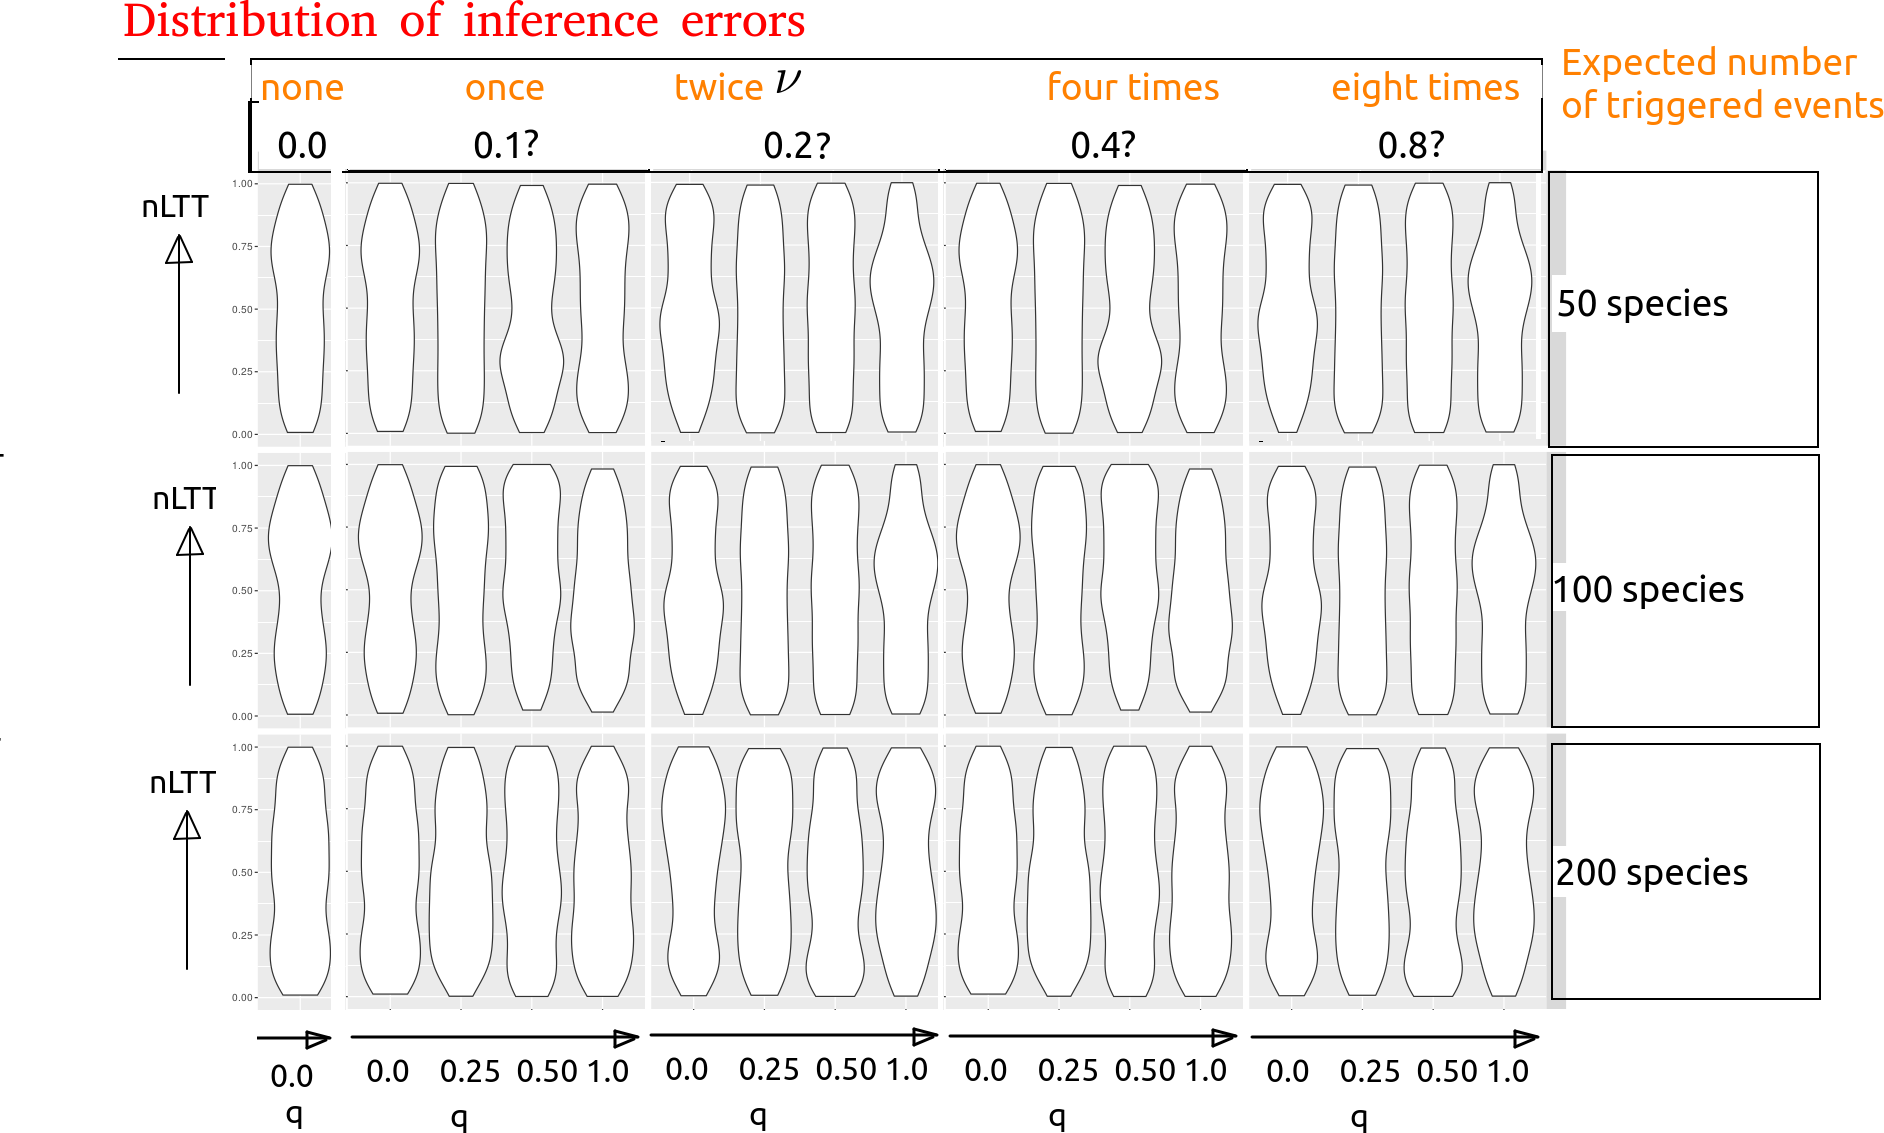
\includegraphics[width=\textwidth]{fig_general.png}
  \caption{
    nLTT statistic distribution per biological parameter set, using the
    general data set, 
    under the (correct) assumptions of a strict clock and Jukes-Cantor site model.
  }
\end{figure}

%%%%%%%%%%%%%%%%%%%%%%%%%%%%%%%%%%%%%%%%%%%%%%%%%%%%%%%%%%%%%%%%%%%%%%%%%%%%%%%%%%%%%%
\section{Glossary}
%%%%%%%%%%%%%%%%%%%%%%%%%%%%%%%%%%%%%%%%%%%%%%%%%%%%%%%%%%%%%%%%%%%%%%%%%%%%%%%%%%%%%%
% Please supply, as a separate list, the definitions of field-specific terms used in your article.
%%%%%%%%%%%%%%%%%%%%%%%%%%%%%%%%%%%%%%%%%%%%%%%%%%%%%%%%%%%%%%%%%%%%%%%%%%%%%%%%
\begin{table}
  \centering 
  \begin{tabular}{l p{0.65\textwidth}}
    \hline
    Term                  & Definition \\
    \hline
    \hline
    Phylogenetics         & The inference of evolutionary relationships of groups of organisms using genetics \\
    Model prior           & Knowledge or assumptions about the ontogeny of evolutionary histories \\
    Posterior             & A collection of phylogenies and parameter estimates, in which more probable combinations (determined by the data and the model prior) are presented more frequently \\
    \hline
  \end{tabular}
  \caption{
    Glossary
  }
  \label{table:glossary}
\end{table}
%%%%%%%%%%%%%%%%%%%%%%%%%%%%%%%%%%%%%%%%%%%%%%%%%%%%%%%%%%%%%%%%%%%%%%%%%%%%%%%%

% Bibliography
%%%%%%%%%%%%%%%%%%%%%%%%%%%%%%%%%%%%%%%%%%%%%%%%%%%%%%%%%%%%%%%%%%%%%%%%%%%%%%%%%%%%%%
% MEE style
\bibliographystyle{mee}
\bibliography{article}
%%%%%%%%%%%%%%%%%%%%%%%%%%%%%%%%%%%%%%%%%%%%%%%%%%%%%%%%%%%%%%%%%%%%%%%%%%%%%%%%%%%%%%

%%%%%%%%%%%%%%%%%%%%%%%%%%%%%%%%%%%%%%%%%%%%%%%%%%%%%%%%%%%%%%%%%%%%%%%%%%%%%%%%%%%%%%
\appendix
%%%%%%%%%%%%%%%%%%%%%%%%%%%%%%%%%%%%%%%%%%%%%%%%%%%%%%%%%%%%%%%%%%%%%%%%%%%%%%%%%%%%%%

\begin{figure}[!htbp]
  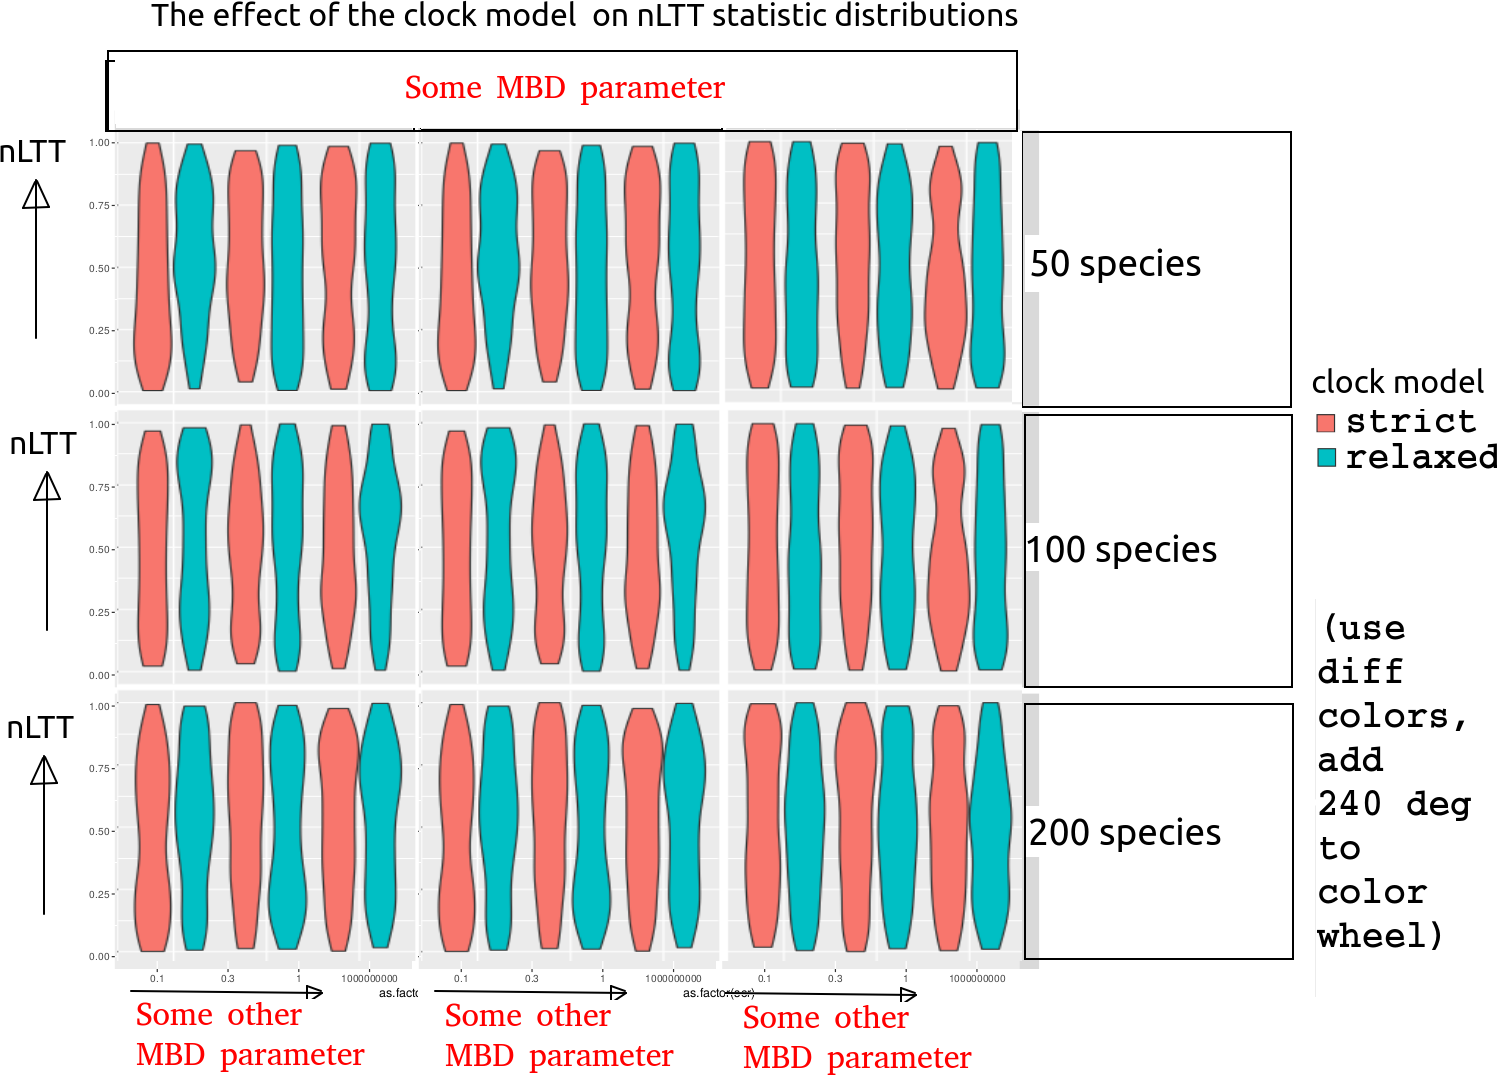
\includegraphics[width=\textwidth]{fig_clock_model.png}
  \caption{
    nLTT statistic distribution per biological parameter set per clock model,
    using the general data set, 
    under the (correct) assumption of a Jukes-Cantor site model.
  }
\end{figure}

\begin{figure}[!htbp]
  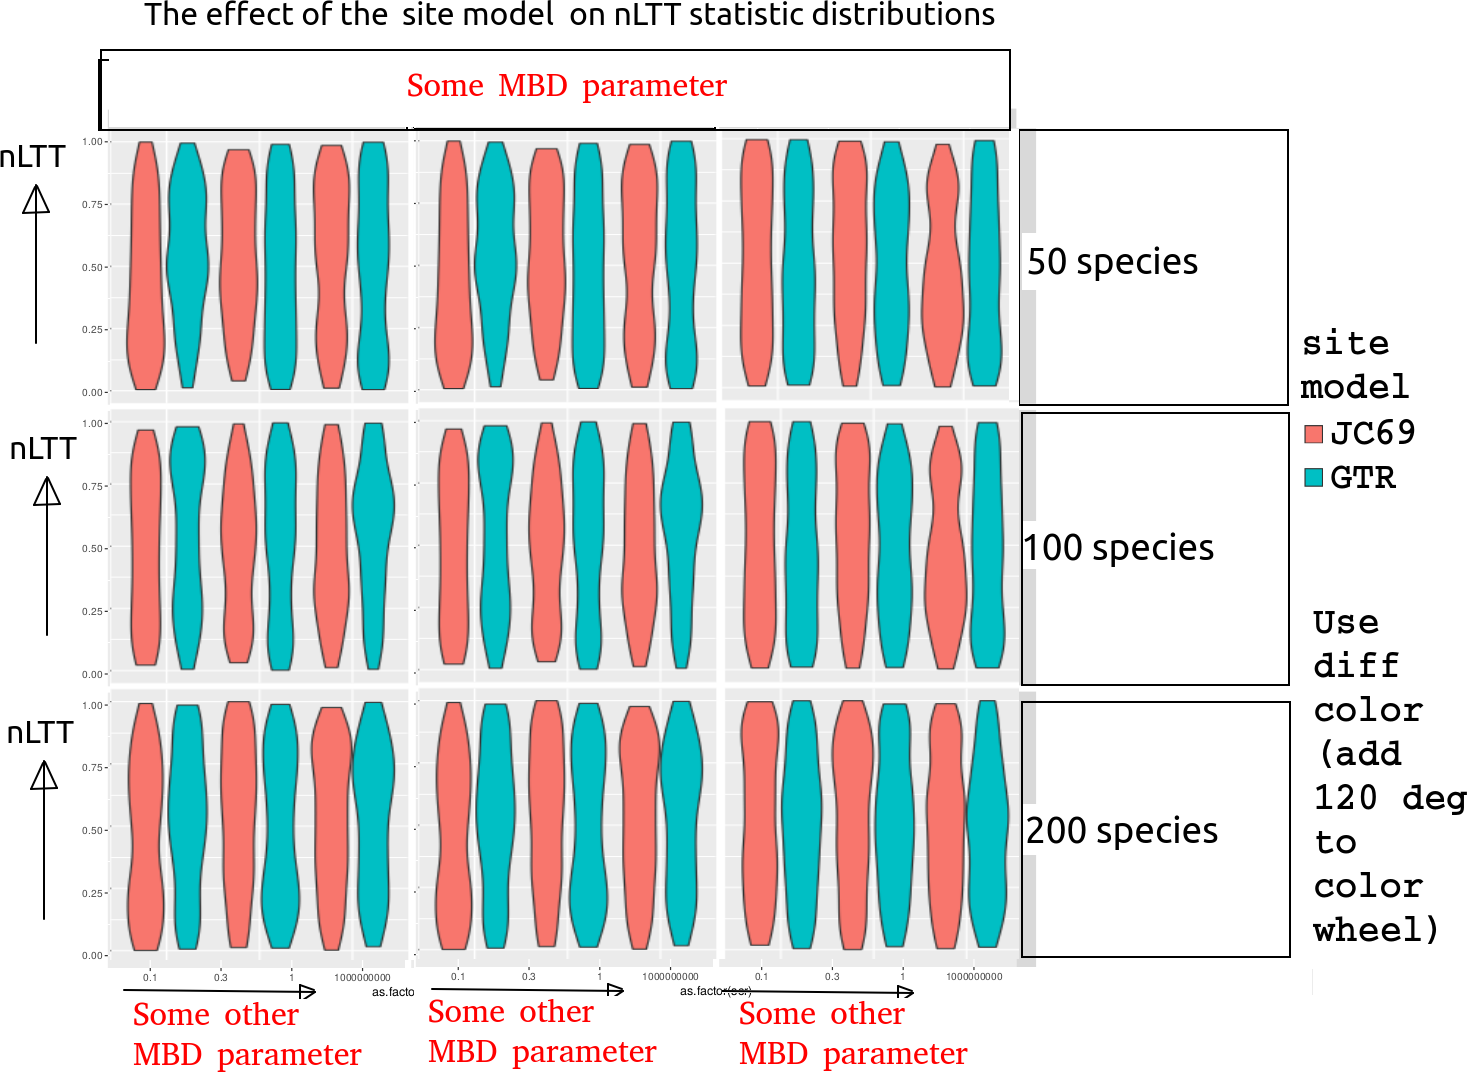
\includegraphics[width=\textwidth]{fig_site_model.png}
  \caption{
    nLTT statistic distribution per biological parameter set per site model,
    using the general data set, 
    under the (correct) assumption of a strict clock model.
  }
\end{figure}

%%%%%%%%%%%%%%%%%%%%%%%%%%%%%%%%%%%%%%%%%%%%%%%%%%%%%%%%%%%%%%%%%%%%%%%%%%%%%%%%
\begin{table}
  \centering 
  \begin{tabular}{p{0.05\textwidth} p{0.6\textwidth} p{0.2\textwidth}}
    \hline
                          & Description & Values \\
    \hline
    \hline
    $\lambda$             & \richel{@gio: MBD params here} & 0.1, 0.3, 1.0, $10^9$ \\
    $\lambda$             & Speciation rate & 0.1, 0.3, 1.0, $10^9$ \\
    $\mu$                 & Extinction rate & 0.0, 0.1, 0.2 \\
    \hline
    $n$                   & Number of good taxa & 50, 100, 200 \\
    $t_c$                 & Crown age & 15 \\
    $\sigma_c$            & Standard deviation around crown age & 0.001 \\
    $M_s$                 & Sampling method & S, L, R \\
    $M_c$                 & Clock model & S, RLN \\
    $M_t$                 & Site model & JC69, GTR \\
    $r$                   & Mutation rate & $\frac{1}{15}$ \\
    $l_a$                 & DNA alignment length & $15K$ \\
    $f_i$                 & MCMC sampling interval & 1K or more \\
    $R_i$                 & RNG seed incipient tree and randomly sampled species tree & 1, 2, etc. \\
    $R_a$                 & RNG seed alignment simulation & $R_i$ \\
    $R_b$                 & RNG seed BEAST2 & $R_i$ \\
    \hline
  \end{tabular}
  \caption{
    Overview of the simulation parameters. Above the horizontal line is 
    the biological parameter set. 
    The RNG seed $R_i$ is 1 for the first simulation, 2 for the next,
    and so on.  
    The clock models are abbreviated as 'S' for a strict and 'RLN' for a relaxed log-normal model.
    The site models are abbreviated as 'JC69' for Jukes-Cantor (\cite{jc69}) and 'GTR' for the generalized 
    time-reversible model (\cite{gtr}).
  }
  \label{table:parameters}
\end{table}
%%%%%%%%%%%%%%%%%%%%%%%%%%%%%%%%%%%%%%%%%%%%%%%%%%%%%%%%%%%%%%%%%%%%%%%%%%%%%%%%

%%%%%%%%%%%%%%%%%%%%%%%%%%%%%%%%%%%%%%%%%%%%%%%%%%%%%%%%%%%%%%%%%%%%%%%%%%%%%%%%
\begin{table}
  \centering 
  \begin{tabular}{l l}
    \hline
    $n$ & Description \\
    \hline
    \hline
    $12$ \richel{recalc} & simulation parameters, see table \ref{table:parameters} \\
    $1000$ & nLTT statistic values \\
    $11$ & ESSes of all parameters estimated by BEAST2 (see specs below) \\
    \hline
  \end{tabular}
  \caption{
    Specification of the data sets. Each row will contain one experiment,
    where the columns contain parameters, measurements and diagnostics.
    This table displays the content of the columns. 
    $n$ denotes the number
    of columns a certain item will occupy, resulting in a table of 
    1023 \richel{recalc} columns and 20K rows.
  }
  \label{table:specs}
\end{table}
%%%%%%%%%%%%%%%%%%%%%%%%%%%%%%%%%%%%%%%%%%%%%%%%%%%%%%%%%%%%%%%%%%%%%%%%%%%%%%%%

%%%%%%%%%%%%%%%%%%%%%%%%%%%%%%%%%%%%%%%%%%%%%%%%%%%%%%%%%%%%%%%%%%%%%%%%%%%%%%%%
\begin{table}
  \centering 
  \begin{tabular}{l l}
    \hline
    \# & Description \\
    \hline
    \hline
    1 & posterior \\
    2 & likelihood \\
    3 & prior \\
    4 & treeLikelihood \\
    5 & TreeHeight \\
    6 & BirthDeath \\
    7 & BDBirthRate \\
    8 & BDDeathRate \\
    9 & logP.mrca \\
    10 & mrcatime \\
    11 & clockRate \\
    \hline
  \end{tabular}
  \caption{
    Overview of the 11 parameters estimated by BEAST2
  }
  \label{table:estimated_parameters}
\end{table}
%%%%%%%%%%%%%%%%%%%%%%%%%%%%%%%%%%%%%%%%%%%%%%%%%%%%%%%%%%%%%%%%%%%%%%%%%%%%%%%%

%%%%%%%%%%%%%%%%%%%%%%%%%%%%%%%%%%%%%%%%%%%%%%%%%%%%%%%%%%%%%%%%%%%%%%%%%%%%%%%%%%%%%%
\section{Acknowledgements}
%%%%%%%%%%%%%%%%%%%%%%%%%%%%%%%%%%%%%%%%%%%%%%%%%%%%%%%%%%%%%%%%%%%%%%%%%%%%%%%%%%%%%%

\richel{put this section here, as the journal does not request for this}
We would like to thank the Center for Information Technology of the University of Groningen for their support
and for providing access to the Peregrine high performance computing cluster.

%%%%%%%%%%%%%%%%%%%%%%%%%%%%%%%%%%%%%%%%%%%%%%%%%%%%%%%%%%%%%%%%%%%%%%%%%%%%%%%%%%%%%%
\section{Authors' contributions}
%%%%%%%%%%%%%%%%%%%%%%%%%%%%%%%%%%%%%%%%%%%%%%%%%%%%%%%%%%%%%%%%%%%%%%%%%%%%%%%%%%%%%%

\richel{put this section here, as the journal does not request for this}
RSE \richel{@gio: I assume this this is true?} conceived the idea for this experiment.
GL created and tested the MBD package.
RJCB created and tested the experiment.
GL and RJCB wrote the first draft of the manuscript. 
RSE contributed substantially to revisions.

\end{document}